\PassOptionsToPackage{unicode=true}{hyperref} % options for packages loaded elsewhere
\PassOptionsToPackage{hyphens}{url}
%
\documentclass[ignorenonframetext,]{beamer}
\usepackage{pgfpages}
\setbeamertemplate{caption}[numbered]
\setbeamertemplate{caption label separator}{: }
\setbeamercolor{caption name}{fg=normal text.fg}
\beamertemplatenavigationsymbolsempty
\usepackage{lmodern}
\usepackage{amssymb,amsmath}
\usepackage{ifxetex,ifluatex}
\usepackage{fixltx2e} % provides \textsubscript
\ifnum 0\ifxetex 1\fi\ifluatex 1\fi=0 % if pdftex
  \usepackage[T1]{fontenc}
  \usepackage[utf8]{inputenc}
  \usepackage{textcomp} % provides euro and other symbols
\else % if luatex or xelatex
  \usepackage{unicode-math}
  \defaultfontfeatures{Ligatures=TeX,Scale=MatchLowercase}
\fi
\usetheme[]{CambridgeUS}
\usecolortheme{beaver}
\usefonttheme{structurebold}
% use upquote if available, for straight quotes in verbatim environments
\IfFileExists{upquote.sty}{\usepackage{upquote}}{}
% use microtype if available
\IfFileExists{microtype.sty}{%
\usepackage[]{microtype}
\UseMicrotypeSet[protrusion]{basicmath} % disable protrusion for tt fonts
}{}
\IfFileExists{parskip.sty}{%
\usepackage{parskip}
}{% else
\setlength{\parindent}{0pt}
\setlength{\parskip}{6pt plus 2pt minus 1pt}
}
\usepackage{hyperref}
\hypersetup{
            pdftitle={B2 - Geokodierung},
            pdfauthor={Jan-Philipp Kolb},
            pdfborder={0 0 0},
            breaklinks=true}
\urlstyle{same}  % don't use monospace font for urls
\newif\ifbibliography
\usepackage{color}
\usepackage{fancyvrb}
\newcommand{\VerbBar}{|}
\newcommand{\VERB}{\Verb[commandchars=\\\{\}]}
\DefineVerbatimEnvironment{Highlighting}{Verbatim}{commandchars=\\\{\}}
% Add ',fontsize=\small' for more characters per line
\usepackage{framed}
\definecolor{shadecolor}{RGB}{42,33,28}
\newenvironment{Shaded}{\begin{snugshade}}{\end{snugshade}}
\newcommand{\AlertTok}[1]{\textcolor[rgb]{1.00,1.00,0.00}{#1}}
\newcommand{\AnnotationTok}[1]{\textcolor[rgb]{0.00,0.40,1.00}{\textbf{\textit{#1}}}}
\newcommand{\AttributeTok}[1]{\textcolor[rgb]{0.74,0.68,0.62}{#1}}
\newcommand{\BaseNTok}[1]{\textcolor[rgb]{0.27,0.67,0.26}{#1}}
\newcommand{\BuiltInTok}[1]{\textcolor[rgb]{0.74,0.68,0.62}{#1}}
\newcommand{\CharTok}[1]{\textcolor[rgb]{0.02,0.61,0.04}{#1}}
\newcommand{\CommentTok}[1]{\textcolor[rgb]{0.00,0.40,1.00}{\textbf{\textit{#1}}}}
\newcommand{\CommentVarTok}[1]{\textcolor[rgb]{0.74,0.68,0.62}{#1}}
\newcommand{\ConstantTok}[1]{\textcolor[rgb]{0.74,0.68,0.62}{#1}}
\newcommand{\ControlFlowTok}[1]{\textcolor[rgb]{0.26,0.66,0.93}{\textbf{#1}}}
\newcommand{\DataTypeTok}[1]{\textcolor[rgb]{0.74,0.68,0.62}{\underline{#1}}}
\newcommand{\DecValTok}[1]{\textcolor[rgb]{0.27,0.67,0.26}{#1}}
\newcommand{\DocumentationTok}[1]{\textcolor[rgb]{0.00,0.40,1.00}{\textit{#1}}}
\newcommand{\ErrorTok}[1]{\textcolor[rgb]{1.00,1.00,0.00}{\textbf{#1}}}
\newcommand{\ExtensionTok}[1]{\textcolor[rgb]{0.74,0.68,0.62}{#1}}
\newcommand{\FloatTok}[1]{\textcolor[rgb]{0.27,0.67,0.26}{#1}}
\newcommand{\FunctionTok}[1]{\textcolor[rgb]{1.00,0.58,0.35}{\textbf{#1}}}
\newcommand{\ImportTok}[1]{\textcolor[rgb]{0.74,0.68,0.62}{#1}}
\newcommand{\InformationTok}[1]{\textcolor[rgb]{0.00,0.40,1.00}{\textbf{\textit{#1}}}}
\newcommand{\KeywordTok}[1]{\textcolor[rgb]{0.26,0.66,0.93}{\textbf{#1}}}
\newcommand{\NormalTok}[1]{\textcolor[rgb]{0.74,0.68,0.62}{#1}}
\newcommand{\OperatorTok}[1]{\textcolor[rgb]{0.74,0.68,0.62}{#1}}
\newcommand{\OtherTok}[1]{\textcolor[rgb]{0.74,0.68,0.62}{#1}}
\newcommand{\PreprocessorTok}[1]{\textcolor[rgb]{0.74,0.68,0.62}{\textbf{#1}}}
\newcommand{\RegionMarkerTok}[1]{\textcolor[rgb]{0.74,0.68,0.62}{#1}}
\newcommand{\SpecialCharTok}[1]{\textcolor[rgb]{0.02,0.61,0.04}{#1}}
\newcommand{\SpecialStringTok}[1]{\textcolor[rgb]{0.02,0.61,0.04}{#1}}
\newcommand{\StringTok}[1]{\textcolor[rgb]{0.02,0.61,0.04}{#1}}
\newcommand{\VariableTok}[1]{\textcolor[rgb]{0.74,0.68,0.62}{#1}}
\newcommand{\VerbatimStringTok}[1]{\textcolor[rgb]{0.02,0.61,0.04}{#1}}
\newcommand{\WarningTok}[1]{\textcolor[rgb]{1.00,1.00,0.00}{\textbf{#1}}}
\usepackage{longtable,booktabs}
\usepackage{caption}
% These lines are needed to make table captions work with longtable:
\makeatletter
\def\fnum@table{\tablename~\thetable}
\makeatother
\usepackage{graphicx,grffile}
\makeatletter
\def\maxwidth{\ifdim\Gin@nat@width>\linewidth\linewidth\else\Gin@nat@width\fi}
\def\maxheight{\ifdim\Gin@nat@height>\textheight\textheight\else\Gin@nat@height\fi}
\makeatother
% Scale images if necessary, so that they will not overflow the page
% margins by default, and it is still possible to overwrite the defaults
% using explicit options in \includegraphics[width, height, ...]{}
\setkeys{Gin}{width=\maxwidth,height=\maxheight,keepaspectratio}
% Prevent slide breaks in the middle of a paragraph:
\widowpenalties 1 10000
\raggedbottom
\setbeamertemplate{part page}{
\centering
\begin{beamercolorbox}[sep=16pt,center]{part title}
  \usebeamerfont{part title}\insertpart\par
\end{beamercolorbox}
}
\setbeamertemplate{section page}{
\centering
\begin{beamercolorbox}[sep=12pt,center]{part title}
  \usebeamerfont{section title}\insertsection\par
\end{beamercolorbox}
}
\setbeamertemplate{subsection page}{
\centering
\begin{beamercolorbox}[sep=8pt,center]{part title}
  \usebeamerfont{subsection title}\insertsubsection\par
\end{beamercolorbox}
}
\AtBeginPart{
  \frame{\partpage}
}
\AtBeginSection{
  \ifbibliography
  \else
    \frame{\sectionpage}
  \fi
}
\AtBeginSubsection{
  \frame{\subsectionpage}
}
\setlength{\emergencystretch}{3em}  % prevent overfull lines
\providecommand{\tightlist}{%
  \setlength{\itemsep}{0pt}\setlength{\parskip}{0pt}}
\setcounter{secnumdepth}{0}

% set default figure placement to htbp
\makeatletter
\def\fps@figure{htbp}
\makeatother


\title{B2 - Geokodierung}
\author{Jan-Philipp Kolb}
\date{23 Oktober 2018}

\begin{document}
\frame{\titlepage}

\begin{frame}{Inhalt dieses Abschnitts}
\protect\hypertarget{inhalt-dieses-abschnitts}{}

\begin{itemize}
\tightlist
\item
  Das Konzept der Geokoordinaten erklären
\item
  Möglichkeiten vorstellen, die Geokodierung mit R durchzuführen
\item
  Nutzung der Nominatim API
\end{itemize}

\end{frame}

\begin{frame}{Geokodierung}
\protect\hypertarget{geokodierung}{}

\begin{block}{\href{https://github.com/adam-p/markdown-here/wiki/Markdown-Cheatsheet\#blockquotes}{Wikipedia
- Geocoding}}

\begin{quote}
Geocoding (\ldots{}) uses a description of a location, most typically a
postal address or place name, to find geographic coordinates from
spatial reference data \ldots{}
\end{quote}

\end{block}

\end{frame}

\begin{frame}[fragile]{Geokodierung mit dem Paket \texttt{ggmap}}
\protect\hypertarget{geokodierung-mit-dem-paket-ggmap}{}

\begin{itemize}
\tightlist
\item
  Einer der ersten Ansätze Geokodierung mit R durchzuführen
\item
  Wenn Geokodierung mit R durchgeführt wird dieses Paket wohl am
  häufigsten verwendet.
\item
  Das führt auch dazu, dass im Internet zahlreiche Anwendungsbeispiele
  zu finden sind.
\end{itemize}

\begin{Shaded}
\begin{Highlighting}[]
\KeywordTok{library}\NormalTok{(ggmap)}
\KeywordTok{geocode}\NormalTok{(}\StringTok{"Heidelberg"}\NormalTok{)}
\end{Highlighting}
\end{Shaded}

\begin{verbatim}
Information from URL : http://maps.googleapis.com/maps/api/geocode/json?address=Heidelberg&sensor=false
       lon      lat
1 8.672434 49.39875
\end{verbatim}

\end{frame}

\begin{frame}{Latitude und Longitude}
\protect\hypertarget{latitude-und-longitude}{}

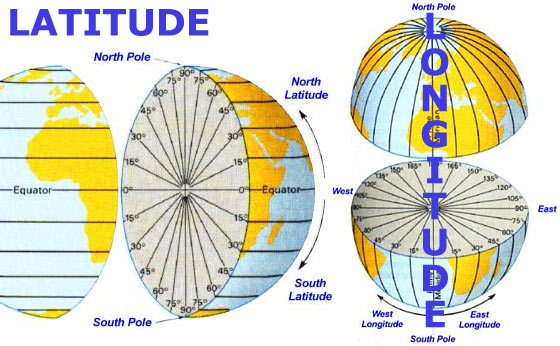
\includegraphics{figure/definition-of-latitude-longitude.jpg}

\href{http://modernsurvivalblog.com/survival-skills/basic-map-reading-latitude-longitude/}{http://modernsurvivalblog.com}

\end{frame}

\begin{frame}[fragile]{Distanzen für verschiedene Verkehrsmittel}
\protect\hypertarget{distanzen-fur-verschiedene-verkehrsmittel}{}

\begin{Shaded}
\begin{Highlighting}[]
\KeywordTok{mapdist}\NormalTok{(}\StringTok{"Q1, 4 Mannheim"}\NormalTok{,}\StringTok{"B2, 1 Mannheim"}\NormalTok{)}
\end{Highlighting}
\end{Shaded}

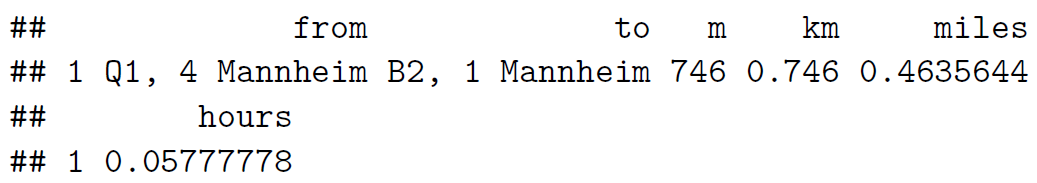
\includegraphics{figure/dist_car.PNG}

\begin{Shaded}
\begin{Highlighting}[]
\KeywordTok{mapdist}\NormalTok{(}\StringTok{"Q1, 4 Mannheim"}\NormalTok{,}\StringTok{"B2, 1 Mannheim"}\NormalTok{,}\DataTypeTok{mode=}\StringTok{"walking"}\NormalTok{)}
\end{Highlighting}
\end{Shaded}

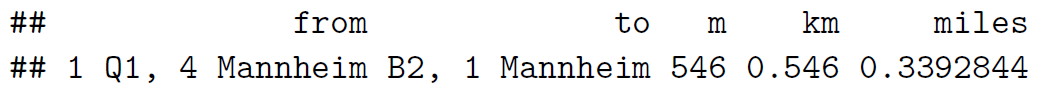
\includegraphics{figure/dist_walking.PNG}

\begin{Shaded}
\begin{Highlighting}[]
\KeywordTok{mapdist}\NormalTok{(}\StringTok{"Q1, 4 Mannheim"}\NormalTok{,}\StringTok{"B2, 1 Mannheim"}\NormalTok{,}\DataTypeTok{mode=}\StringTok{"bicycling"}\NormalTok{)}
\end{Highlighting}
\end{Shaded}

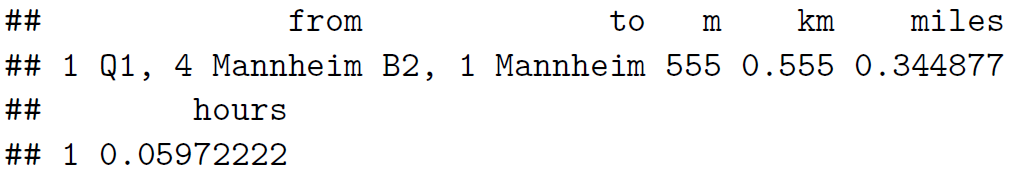
\includegraphics{figure/dist_bike.PNG}

\end{frame}

\begin{frame}[fragile]{Geokodierung mit dem Paket \texttt{tmaptools}}
\protect\hypertarget{geokodierung-mit-dem-paket-tmaptools}{}

\begin{itemize}
\tightlist
\item
  Beim Paket \texttt{tmaptools} wird die Nominatim API zur Geokodierung
  verwendet.
\item
  Diese Funktion hat den Vorteil, dass eine Projektion ausgewählt werden
  kann, in der die Geokodierungen zurück gegeben werden.
\end{itemize}

\begin{Shaded}
\begin{Highlighting}[]
\KeywordTok{library}\NormalTok{(}\StringTok{"tmaptools"}\NormalTok{)}
\end{Highlighting}
\end{Shaded}

\begin{Shaded}
\begin{Highlighting}[]
\NormalTok{?geocode_OSM}
\end{Highlighting}
\end{Shaded}

\end{frame}

\begin{frame}[fragile]{Koordinaten verschiedener Orte in Deutschland}
\protect\hypertarget{koordinaten-verschiedener-orte-in-deutschland}{}

\begin{block}{Geokodierung mit einer Schleife}

\begin{Shaded}
\begin{Highlighting}[]
\NormalTok{cities <-}\StringTok{ }\KeywordTok{c}\NormalTok{(}\StringTok{"Hamburg"}\NormalTok{,}\StringTok{"Koeln"}\NormalTok{,}\StringTok{"Dresden"}\NormalTok{,}\StringTok{"Muenchen"}\NormalTok{)}

\NormalTok{lat <-}\StringTok{ }\KeywordTok{vector}\NormalTok{()}
\NormalTok{lon <-}\StringTok{ }\KeywordTok{vector}\NormalTok{()}
\ControlFlowTok{for}\NormalTok{ (i }\ControlFlowTok{in} \DecValTok{1}\OperatorTok{:}\KeywordTok{length}\NormalTok{(cities))\{}
\NormalTok{  gc <-}\StringTok{ }\KeywordTok{geocode_OSM}\NormalTok{(cities[i])}
\NormalTok{  lat[i] <-}\StringTok{ }\NormalTok{gc}\OperatorTok{$}\NormalTok{coords[}\DecValTok{1}\NormalTok{]}
\NormalTok{  lon[i] <-}\StringTok{ }\NormalTok{gc}\OperatorTok{$}\NormalTok{coords[}\DecValTok{2}\NormalTok{]}
\NormalTok{\}}
\end{Highlighting}
\end{Shaded}

\end{block}

\end{frame}

\begin{frame}[fragile]{Welche Koordinaten hat der Norden}
\protect\hypertarget{welche-koordinaten-hat-der-norden}{}

\begin{Shaded}
\begin{Highlighting}[]
\NormalTok{Dat <-}\StringTok{ }\KeywordTok{data.frame}\NormalTok{(cities,lon,lat)}
\KeywordTok{kable}\NormalTok{(Dat)}
\end{Highlighting}
\end{Shaded}

\begin{longtable}[]{@{}lrr@{}}
\toprule
cities & lon & lat\tabularnewline
\midrule
\endhead
Hamburg & 53.55034 & 10.000654\tabularnewline
Koeln & 50.93836 & 6.959974\tabularnewline
Dresden & 51.04933 & 13.738144\tabularnewline
Muenchen & 48.13711 & 11.575382\tabularnewline
\bottomrule
\end{longtable}

\end{frame}

\begin{frame}[fragile]{Reverse Geokodierung}
\protect\hypertarget{reverse-geokodierung}{}

\begin{quote}
Reverse geocoding is the process of back (reverse) coding of a point
location (latitude, longitude) to a readable address or place name. This
permits the identification of nearby street addresses, places, and/or
areal subdivisions such as neighbourhoods, county, state, or country.
\end{quote}

Quelle:
\href{https://en.wikipedia.org/wiki/Reverse_geocoding}{Wikipedia}

\begin{Shaded}
\begin{Highlighting}[]
\KeywordTok{revgeocode}\NormalTok{(}\KeywordTok{c}\NormalTok{(}\DecValTok{48}\NormalTok{,}\DecValTok{8}\NormalTok{))}
\end{Highlighting}
\end{Shaded}

\end{frame}

\begin{frame}[fragile]{Daten einlesen}
\protect\hypertarget{daten-einlesen}{}

\begin{itemize}
\tightlist
\item
  Hier wird ein Beispieldatensatz eingelesen, den ich über räumliche
  Stichproben und reverse geocoding erzeugt habe.
\end{itemize}

\begin{Shaded}
\begin{Highlighting}[]
\KeywordTok{load}\NormalTok{(}\StringTok{"../data/addr_list_t_68239.RData"}\NormalTok{)}
\KeywordTok{head}\NormalTok{(addr_list_t)}
\end{Highlighting}
\end{Shaded}

\begin{verbatim}
## [1] "Lilienstraße 32A, 68535 Edingen-Neckarhausen, Germany"
## [2] "Waldspitze 6, 68239 Mannheim, Germany"                
## [3] "Holzweg 51, 68239 Mannheim, Germany"                  
## [4] "Kloppenheimer Str. 247, 68239 Mannheim, Germany"      
## [5] "Mallaustraße 121, 68219 Mannheim, Germany"            
## [6] "Holzweg 33A, 68239 Mannheim, Germany"
\end{verbatim}

\end{frame}

\begin{frame}[fragile]{Die erste Adressen geokodieren}
\protect\hypertarget{die-erste-adressen-geokodieren}{}

\begin{Shaded}
\begin{Highlighting}[]
\KeywordTok{geocode_OSM}\NormalTok{(addr_list_t[}\DecValTok{1}\NormalTok{])}
\end{Highlighting}
\end{Shaded}

\begin{verbatim}
## $query
## [1] "Lilienstraße 32A, 68535 Edingen-Neckarhausen, Germany"
## 
## $coords
##         x         y 
##  8.584601 49.445360 
## 
## $bbox
##         min       max
## x  8.584494  8.584708
## y 49.445276 49.445443
\end{verbatim}

\end{frame}

\begin{frame}[fragile]{Alle Adressen geokodieren}
\protect\hypertarget{alle-adressen-geokodieren}{}

\begin{itemize}
\tightlist
\item
  im Objekt \texttt{gc\_list} werden die Ergebnisse gespeichert.
\end{itemize}

\begin{Shaded}
\begin{Highlighting}[]
\NormalTok{gc_list <-}\StringTok{ }\KeywordTok{list}\NormalTok{()}

\ControlFlowTok{for}\NormalTok{ (i }\ControlFlowTok{in} \DecValTok{1}\OperatorTok{:}\KeywordTok{length}\NormalTok{(addr_list_t))\{}
\NormalTok{  gc_list[[i]] <-}\StringTok{ }\KeywordTok{geocode_OSM}\NormalTok{(addr_list_t[i])}
\NormalTok{\}}
\end{Highlighting}
\end{Shaded}

\end{frame}

\begin{frame}[fragile]{Geokodierung mit dem R-Paket \texttt{opencage}}
\protect\hypertarget{geokodierung-mit-dem-r-paket-opencage}{}

\begin{itemize}
\tightlist
\item
  Um dieses Paket zu nutzen muss man sich vorher bei der API
  registrieren
\end{itemize}

\begin{Shaded}
\begin{Highlighting}[]
\KeywordTok{library}\NormalTok{(opencage)}
\end{Highlighting}
\end{Shaded}

\begin{Shaded}
\begin{Highlighting}[]
\NormalTok{gc_info<-}\KeywordTok{opencage_forward}\NormalTok{(}\DataTypeTok{placename =} 
                              \StringTok{"Amsterdam, Van Woustraat"}\NormalTok{)}
\end{Highlighting}
\end{Shaded}

\begin{itemize}
\tightlist
\item
  Hinweise, wie das Paket genutzt erden kann sind im
  \href{https://ropensci.org/tutorials/opencage_tutorial/}{\textbf{opencage
  Tutorial}} zu finden.
\end{itemize}

\end{frame}

\begin{frame}[fragile]{Das Paket
\href{https://github.com/ropensci/geonames}{\texttt{geonames}}}
\protect\hypertarget{das-paket-geonames}{}

\begin{block}{Nutzung des \texttt{geonames} Paketes}

\begin{itemize}
\tightlist
\item
  Ein Account ist notwendig um die meisten Funktionen des Paketes
  \texttt{geonames}zu nutzen.
\end{itemize}

\begin{Shaded}
\begin{Highlighting}[]
\KeywordTok{library}\NormalTok{(geonames)}
\end{Highlighting}
\end{Shaded}

\begin{Shaded}
\begin{Highlighting}[]
\KeywordTok{options}\NormalTok{(}\DataTypeTok{geonamesUsername=}\StringTok{"myusername"}\NormalTok{)}
\end{Highlighting}
\end{Shaded}

\begin{Shaded}
\begin{Highlighting}[]
\NormalTok{MAwiki<-}\KeywordTok{GNfindNearbyWikipedia}\NormalTok{(}\DataTypeTok{postalcode=}\DecValTok{68239}\NormalTok{,}\DataTypeTok{country=}\StringTok{"DE"}\NormalTok{,}
                              \DataTypeTok{radius=}\DecValTok{10}\NormalTok{)}
\end{Highlighting}
\end{Shaded}

\end{block}

\end{frame}

\begin{frame}{Beispiel Geonames}
\protect\hypertarget{beispiel-geonames}{}

\begin{block}{Wikipediaeinträge in der Nähe}

\begin{itemize}
\item
  \href{http://www.geonames.org/login}{\textbf{Login}} für die Nutzung
  des Web-Services Geonames.
\item
  \href{http://www.geonames.org/enablefreewebservice}{\textbf{Hier}}
  kann man das Arbeiten mit dem Webservice starten.
\item
  \href{http://www.geonames.org/export/ws-overview.html}{\textbf{Informationen
  zum Download bei Geonames}}
\end{itemize}

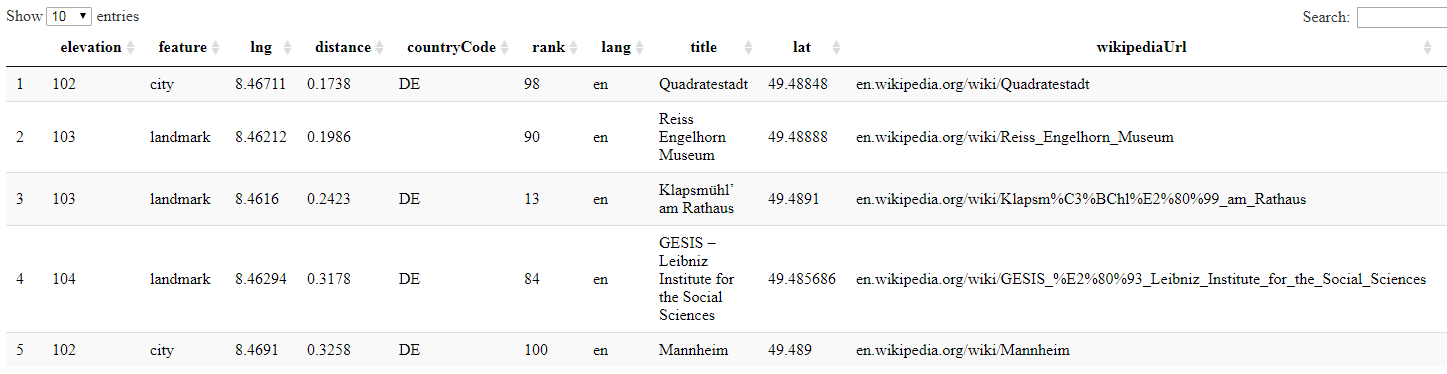
\includegraphics{figure/Wiki_Mannheim.PNG}

\end{block}

\end{frame}

\begin{frame}[fragile]{Eine Bounding Box erstellen}
\protect\hypertarget{eine-bounding-box-erstellen}{}

\begin{Shaded}
\begin{Highlighting}[]
\KeywordTok{library}\NormalTok{(osmdata)}
\NormalTok{bbox <-}\StringTok{ }\KeywordTok{getbb}\NormalTok{(}\StringTok{"Mannheim"}\NormalTok{)}
\end{Highlighting}
\end{Shaded}

\begin{Shaded}
\begin{Highlighting}[]
\NormalTok{erg <-}\StringTok{ }\NormalTok{geonames}\OperatorTok{::}\KeywordTok{GNcities}\NormalTok{(}\FloatTok{49.649591}\NormalTok{,}\FloatTok{8.627236}\NormalTok{,}
                          \FloatTok{49.329591}\NormalTok{,}\FloatTok{8.307236}\NormalTok{)}
\end{Highlighting}
\end{Shaded}

\end{frame}

\begin{frame}[fragile]{Geokodieren mit der API Nominatim}
\protect\hypertarget{geokodieren-mit-der-api-nominatim}{}

\begin{block}{Zunächst muss der Link erzeugt werden}

\begin{Shaded}
\begin{Highlighting}[]
\KeywordTok{library}\NormalTok{(}\StringTok{"RJSONIO"}\NormalTok{)}
\NormalTok{api_adress <-}\StringTok{ "http://nominatim.openstreetmap.org/search?format="}
\NormalTok{file_format <-}\StringTok{ "json"}
\NormalTok{search_query <-}\StringTok{ "&addressdetails=1&extratags=1&q="}
\NormalTok{adress <-}\StringTok{ "Amsterdam+Niederlande+Rozengracht+1"}

\NormalTok{link <-}\StringTok{ }\KeywordTok{paste0}\NormalTok{(api_adress,file_format,search_query,adress)}
\NormalTok{link}
\end{Highlighting}
\end{Shaded}

\begin{verbatim}
## [1] "http://nominatim.openstreetmap.org/search?format=json&addressdetails=1&extratags=1&q=Amsterdam+Niederlande+Rozengracht+1"
\end{verbatim}

\end{block}

\end{frame}

\begin{frame}[fragile]{Der Download mit Nominatim}
\protect\hypertarget{der-download-mit-nominatim}{}

\begin{Shaded}
\begin{Highlighting}[]
\NormalTok{con <-}\StringTok{ }\KeywordTok{url}\NormalTok{(link)}
\NormalTok{geoc <-}\StringTok{ }\KeywordTok{fromJSON}\NormalTok{(}\KeywordTok{paste}\NormalTok{(}\KeywordTok{readLines}\NormalTok{(con,}\DataTypeTok{warn=}\NormalTok{F), }
                       \DataTypeTok{collapse =} \StringTok{''}\NormalTok{))}
\KeywordTok{close}\NormalTok{(con)}
\end{Highlighting}
\end{Shaded}

\end{frame}

\begin{frame}[fragile]{So sieht das Ergebnis aus}
\protect\hypertarget{so-sieht-das-ergebnis-aus}{}

\begin{Shaded}
\begin{Highlighting}[]
\KeywordTok{names}\NormalTok{(geoc[[}\DecValTok{1}\NormalTok{]])}
\end{Highlighting}
\end{Shaded}

\begin{verbatim}
##  [1] "place_id"     "licence"      "osm_type"     "osm_id"      
##  [5] "boundingbox"  "lat"          "lon"          "display_name"
##  [9] "class"        "type"         "importance"   "address"     
## [13] "extratags"
\end{verbatim}

\begin{Shaded}
\begin{Highlighting}[]
\NormalTok{geoc[[}\DecValTok{1}\NormalTok{]]}\OperatorTok{$}\NormalTok{address}
\end{Highlighting}
\end{Shaded}

\begin{verbatim}
##    house_number            road     residential          suburb 
##             "1"   "Rozengracht"       "Jordaan"     "Amsterdam" 
##   city_district            city           state        postcode 
##       "Centrum"     "Amsterdam" "Noord-Holland"        "1016LP" 
##         country    country_code 
##     "Nederland"            "nl"
\end{verbatim}

\end{frame}

\begin{frame}[fragile]{Das Paket \texttt{jsonlite} nutzen}
\protect\hypertarget{das-paket-jsonlite-nutzen}{}

\begin{Shaded}
\begin{Highlighting}[]
\NormalTok{con <-}\StringTok{ }\KeywordTok{url}\NormalTok{(}\StringTok{"http://nominatim.openstreetmap.org/search?format=json&}
\StringTok{           addressdetails=1&extratags=1&q=Amsterdam+Niederlande+Rozengracht+1"}\NormalTok{)}
\NormalTok{geoc2 <-}\StringTok{ }\NormalTok{jsonlite}\OperatorTok{::}\KeywordTok{fromJSON}\NormalTok{(con)}

\NormalTok{geoc2df <-}\StringTok{ }\KeywordTok{with}\NormalTok{(geoc2,}\KeywordTok{data.frame}\NormalTok{(osm_id,lat,lon))}
\NormalTok{geoc2df}\OperatorTok{$}\NormalTok{house_number <-}\StringTok{  }\NormalTok{geoc2}\OperatorTok{$}\NormalTok{address}\OperatorTok{$}\NormalTok{house_number}
\end{Highlighting}
\end{Shaded}

Wir erhalten nun Daten für mehrere Anschriften:

\begin{longtable}[]{@{}llll@{}}
\toprule
osm\_id & lat & lon & house\_number\tabularnewline
\midrule
\endhead
2721815875 & 52.3737223 & 4.8826404 & 1\tabularnewline
2743624072 & 52.3719482 & 4.8755534 & 237-1\tabularnewline
2721830930 & 52.3736673 & 4.8823914 & 7-1\tabularnewline
2721827922 & 52.3734021 & 4.8813371 & 53-1\tabularnewline
2721824637 & 52.372232 & 4.8767542 & 231-1\tabularnewline
2721823434 & 52.3724786 & 4.8776618 & 187-1\tabularnewline
2721820122 & 52.3727335 & 4.8786657 & 137-1\tabularnewline
2721816644 & 52.3729874 & 4.8797588 & 105E-1\tabularnewline
2720971311 & 52.3727658 & 4.8775263 & 194-1\tabularnewline
2720971056 & 52.3728019 & 4.8775994 & 184-1\tabularnewline
\bottomrule
\end{longtable}

\end{frame}

\begin{frame}[fragile]{Das Paket \texttt{googleway}}
\protect\hypertarget{das-paket-googleway}{}

\begin{quote}
Accesses Google Maps APIs to Retrieve Data and Plot Maps
\end{quote}

\begin{Shaded}
\begin{Highlighting}[]
\KeywordTok{library}\NormalTok{(googleway)}
\end{Highlighting}
\end{Shaded}

\begin{itemize}
\tightlist
\item
  Ein API Schlüssel ist notwendig um die meisten Funktionen des Paketes
  zu nutzen.
\end{itemize}

\end{frame}

\begin{frame}[fragile]{Das Paket \texttt{bbox}}
\protect\hypertarget{das-paket-bbox}{}

\begin{itemize}
\item
  Das Paket \texttt{bbox} ist auf github zu finden.
\item
  Beispieldatensatz laden:
\end{itemize}

\begin{Shaded}
\begin{Highlighting}[]
\KeywordTok{load}\NormalTok{(}\StringTok{"../data/ddat.RData"}\NormalTok{)}
\end{Highlighting}
\end{Shaded}

\begin{itemize}
\tightlist
\item
  Rahmen für das räumliche Objekt bestimmen:
\end{itemize}

\begin{Shaded}
\begin{Highlighting}[]
\KeywordTok{library}\NormalTok{(bbox)}
\KeywordTok{b_box}\NormalTok{(ddat)}
\end{Highlighting}
\end{Shaded}

\begin{verbatim}
## [1]  5.866286 47.273602 15.048632 55.058262
\end{verbatim}

\begin{Shaded}
\begin{Highlighting}[]
\KeywordTok{citation}\NormalTok{(}\StringTok{"bbox"}\NormalTok{)}
\end{Highlighting}
\end{Shaded}

\end{frame}

\begin{frame}[fragile]{Links}
\protect\hypertarget{links}{}

\begin{itemize}
\item
  Überblick von Jesse Sadler zur
  \href{https://www.jessesadler.com/post/geocoding-with-r/}{\textbf{Geokodierung
  mit R}}
\item
  Ein Schummelzettel für
  \href{https://www.nceas.ucsb.edu/~frazier/RSpatialGuides/ggmap/ggmapCheatsheet.pdf}{\textbf{\texttt{ggmap}}}
\item
  Die Vignette zum Paket \texttt{tmap} -
  \href{https://cran.r-project.org/web/packages/tmap/vignettes/tmap-getstarted.html}{\textbf{tmap:
  get started}}
\item
  \href{https://www.latlong.net/place/hamburg-germany-8766.html}{\textbf{latlong.net}}
  - eine Homepage um Koordinaaten zu bestimmen.
\end{itemize}

\end{frame}

\end{document}
